% answers.tex —— 1977 年·安徽卷（理科） · 参考答案与详细解析片段
% 由 tools/generate_projects.py 依来源总账自 1977/1977_数学真题_安徽理_试题.md + 1977/1977_数学真题_安徽理_解析正文.md + 1977/1977_数学真题_安徽理_答案要点.md 生成，勿手改（改源 MD 后重跑）


\begin{gktip}
固定源卷第 5—13 页附「解答及评分标准（原试题均略）」。下文逐题独立推导，并对照源解答复核关键结论。第 1(1) 题原卷跨行处行末、行首重复印出的加号按一个加号计算；第 1(6) 题题面印作 sinA 而源解答按 secA 展开，两处不一致，下文按题面口径化简并附源口径结果；第 4(2) 题数列的分母依次为 $3,\ 3^2,\ 3^4,\ 3^8,\ \cdots$（指数为 2 的幂），已按 600 dpi 局部放大与源解答双重确认；第 8 题原卷「1.」「2.」已重排为（1）（2）；原卷未编号的〔附加题〕编为附加题 9。
\end{gktip}

\begin{answer}
\gksolhead{1}{}

\textbf{题目}（本题满分 20 分，每小题 3 分）：

\begin{gktip}
\textbf{源注}：原卷题首即标注「本题满分20分，每小题3分」；7 个小题按每小题 3 分计应为 21 分，与满分 20 分不一致，源卷两数并存，本文照录。
\end{gktip}

\Needspace{5\baselineskip}
（1） 计算：

\nopagebreak[4]
\[
0.25\times(-2)^2-4\div(\sqrt5-1)^0-\left(\frac16\right)^{-\frac12}+
\]

\nopagebreak[4]
\[
+\frac{\sqrt3}{\sqrt3-\sqrt2};
\]

\begin{gktip}
\textbf{源注}：原卷此式跨行排印，行末与行首各印一个加号；按数学含义应只有一个加号，本文两处照录，计算按一个加号处理（源解答亦如此）。
\end{gktip}

（2） 求函数 $y=\log_a(4^x-16)$ 的定义域；

（3） 求 $\sin(-915^\circ)$ 的值；

（4） 求函数 $y=\arcsin(1-2x)$ 的定义域；

（5） 化复数 $-1+i$ 为三角函数式；

（6） 化简 $\sin A\cdot\sqrt{1-\sin^2A}$ （$90^\circ<A\leqslant180^\circ$）

\begin{gktip}
\textbf{源注}：原卷题面印作「sinA·√(1$-$sin²A)」，源卷解答部分却按「secA·√(1$-$sin²A)」展开并得 $-$1，两处不一致；本文按题面照录，解析中按题面化简并附源解答口径的结果。
\end{gktip}

（7） 已知元锥的母线长 3 cm，底面直径 2 cm，求它的侧面积（$\pi$ 取 3.14）。

\begin{gktip}
\textbf{源注}：「元锥」为原卷用字（源解答部分作「园锥」），即圆锥，本文照录。
\end{gktip}

\Needspace{4\baselineskip}
\textbf{解析}

\gksubpart{（1）}

\Needspace{5\baselineskip}
按一个加号计算。逐项求值：

\nopagebreak[4]
\[
0.25\times(-2)^2=0.25\times4=1,
\qquad
4\div(\sqrt5-1)^0=4\div1=4,
\]

\nopagebreak[4]
\[
\left(\frac16\right)^{-\frac12}=6^{\frac12}=\sqrt6,
\]

\Needspace{5\baselineskip}
分母有理化：

\nopagebreak[4]
\[
\frac{\sqrt3}{\sqrt3-\sqrt2}
=\frac{\sqrt3(\sqrt3+\sqrt2)}{(\sqrt3-\sqrt2)(\sqrt3+\sqrt2)}
=\frac{3+\sqrt6}{3-2}=3+\sqrt6.
\]

\Needspace{5\baselineskip}
所以

\nopagebreak[4]
\[
\text{\text{原式}}=1-4-\sqrt6+(3+\sqrt6)=0.
\]

\gksubpart{（2）}

\Needspace{5\baselineskip}
真数须为正，且对数的底 $a>0$、$a\ne1$。由

\nopagebreak[4]
\[
4^x-16>0
\quad\Longrightarrow\quad
4^x>4^2,
\]

\Needspace{5\baselineskip}
得定义域为

\nopagebreak[4]
\[
x>2.
\]

\gksubpart{（3）}

\nopagebreak[4]
\[
\sin(-915^\circ)=-\sin915^\circ
=-\sin(2\times360^\circ+195^\circ)
=-\sin195^\circ.
\]

\Needspace{5\baselineskip}
而 $195^\circ=180^\circ+15^\circ$，故 $\sin195^\circ=-\sin15^\circ$，于是

\nopagebreak[4]
\[
\sin(-915^\circ)=\sin15^\circ
=\sin(45^\circ-30^\circ)
=\frac{\sqrt6-\sqrt2}{4}.
\]

\gksubpart{（4）}

\Needspace{5\baselineskip}
要使 $\arcsin(1-2x)$ 有意义，必须

\nopagebreak[4]
\[
-1\leqslant1-2x\leqslant1,
\]

\Needspace{5\baselineskip}
解得

\nopagebreak[4]
\[
0\leqslant x\leqslant1.
\]

\gksubpart{（5）}

\Needspace{5\baselineskip}
复数 $-1+i$ 的模为 $\sqrt{(-1)^2+1^2}=\sqrt2$，对应的点在第二象限，辐角主值为

\nopagebreak[4]
\[
\pi-\frac{\pi}{4}=\frac{3\pi}{4}.
\]

\Needspace{5\baselineskip}
所以三角函数式为

\nopagebreak[4]
\[
-1+i=\sqrt2\left(\cos\frac{3\pi}{4}+i\sin\frac{3\pi}{4}\right).
\]

\gksubpart{（6）}

\Needspace{5\baselineskip}
按题面化简。由 $90^\circ<A\leqslant180^\circ$ 得 $\cos A<0$，故

\nopagebreak[4]
\[
\sqrt{1-\sin^2A}=\sqrt{\cos^2A}=|\cos A|=-\cos A,
\]

\Needspace{5\baselineskip}
于是

\nopagebreak[4]
\[
\sin A\cdot\sqrt{1-\sin^2A}
=\sin A\cdot(-\cos A)
=-\sin A\cos A
=-\frac12\sin2A.
\]

\begin{gktip}
\textbf{源注复核}：源卷解答此小题印作「按 seCA·√(1$-$sin²A)」展开，即按 $\sec A\cdot\sqrt{1-\sin^2A}=\sec A\cdot(-\cos A)=-1$ 计算，与题面印刷的 sinA 不一致。本文以题面为准给出 $-\dfrac12\sin2A$，并附源口径结果 $-1$；源卷两处孰为排印之误，未能确认。
\end{gktip}

\gksubpart{（7）}

\Needspace{5\baselineskip}
底面直径 $2$ cm，则底面半径 $r=1$ cm；母线 $l=3$ cm。圆锥侧面积

\nopagebreak[4]
\[
S_{\text{\text{侧}}}=\pi rl=3.14\times1\times3=9.42\ (\mathrm{cm^2}).
\]

\gkanswer{答案（1）：$0$。}

\gkanswer{答案（2）：$x>2$。}

\gkanswer{答案（3）：$\dfrac{\sqrt6-\sqrt2}{4}$。}

\gkanswer{答案（4）：$0\leqslant x\leqslant1$。}

\gkanswer{答案（5）：$\sqrt2\left(\cos\dfrac{3\pi}{4}+i\sin\dfrac{3\pi}{4}\right)$。}

\gkanswer{答案（6）：按题面为 $-\sin A\cos A=-\dfrac12\sin2A$；源解答按 $\sec A$ 口径得 $-1$（见解析）。}

\gkanswer{答案（7）：$9.42\ \mathrm{cm^2}$。}

\end{answer}
\begin{answer}
\gksolhead{2}{}

\textbf{题目}（本题 9 分）：

用宽为 80 厘米的铁皮制作一个槽，槽的截面 $ABCD$ 是一个矩形。

（1） 求槽的截面积 $y$ 关于槽深 $x$ 的函数关系式；

（2） 求出这个函数圆象的顶点坐标、对称轴方程；

\begin{gktip}
\textbf{源注}：原卷印作「函数圆象」，应为「图象」之误排，本文照录。
\end{gktip}

（3） 当槽深为多少厘米时，槽的截面积最大？这个最大面积是多少平方厘米？

\begin{gktip}
原源 PDF 第 2 页题首附有槽的立体示意图（旁注「安，二」）；LaTeX 版按源图重绘。
\end{gktip}
\nopagebreak[4]
\begin{center}% 1977 年安徽卷（理科）第 2 题：铁皮槽立体示意图，截面矩形 ABCD（A 左上、B 左下、C 右下、D 右上），
% 槽口两斜棱在远端交汇，其间按原卷标注 π/6 角（按源卷第 2 页「安，二」图布局重绘）
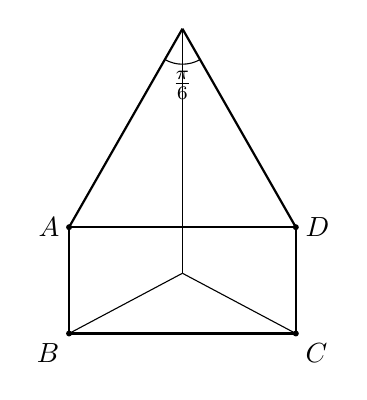
\begin{tikzpicture}[scale=0.9]
  % 前面板矩形
  \coordinate (A) at (0,1.5);
  \coordinate (B) at (0,0);
  \coordinate (C) at (3.2,0);
  \coordinate (D) at (3.2,1.5);
  % 远端顶点（手绘原图将远端上下棱各收缩为一点）
  \coordinate (P) at (1.6,4.3);
  \coordinate (Q) at (1.6,0.85);
  \draw[thick] (A)--(B)--(C)--(D);
  \draw[thick] (A)--(P);
  \draw[thick] (D)--(P);
  \draw[thin]  (B)--(Q);
  \draw[thin]  (C)--(Q);
  \draw[thin]  (P)--(Q);
  \draw[thick] (A)--(D);
  \fill (A) circle (1.2pt) node[left] {$A$};
  \fill (B) circle (1.2pt) node[below left] {$B$};
  \fill (C) circle (1.2pt) node[below right] {$C$};
  \fill (D) circle (1.2pt) node[right] {$D$};
  % 槽口两斜棱夹角标注（原卷标注 π/6，题面与解答未使用，按原样保留）
  \draw (P) ++(240.3:0.5) arc[start angle=240.3, end angle=299.7, radius=0.5];
  \node at (1.6,3.5) {$\frac{\pi}{6}$};
\end{tikzpicture}
\end{center}
\nopagebreak[4]
\Needspace{4\baselineskip}
\textbf{解析}

铁皮宽 $80$ 厘米，折成矩形截面 $ABCD$：两侧壁深均为槽深 $x$，底边宽为 $80-2x$（$0<x<40$）。
\nopagebreak[4]
\begin{center}% 1977 年安徽卷（理科）第 2 题：铁皮槽立体示意图，截面矩形 ABCD（A 左上、B 左下、C 右下、D 右上），
% 槽口两斜棱在远端交汇，其间按原卷标注 π/6 角（按源卷第 2 页「安，二」图布局重绘）
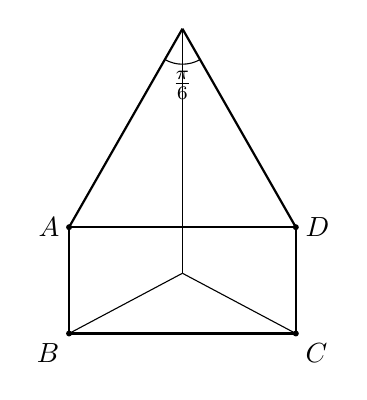
\begin{tikzpicture}[scale=0.9]
  % 前面板矩形
  \coordinate (A) at (0,1.5);
  \coordinate (B) at (0,0);
  \coordinate (C) at (3.2,0);
  \coordinate (D) at (3.2,1.5);
  % 远端顶点（手绘原图将远端上下棱各收缩为一点）
  \coordinate (P) at (1.6,4.3);
  \coordinate (Q) at (1.6,0.85);
  \draw[thick] (A)--(B)--(C)--(D);
  \draw[thick] (A)--(P);
  \draw[thick] (D)--(P);
  \draw[thin]  (B)--(Q);
  \draw[thin]  (C)--(Q);
  \draw[thin]  (P)--(Q);
  \draw[thick] (A)--(D);
  \fill (A) circle (1.2pt) node[left] {$A$};
  \fill (B) circle (1.2pt) node[below left] {$B$};
  \fill (C) circle (1.2pt) node[below right] {$C$};
  \fill (D) circle (1.2pt) node[right] {$D$};
  % 槽口两斜棱夹角标注（原卷标注 π/6，题面与解答未使用，按原样保留）
  \draw (P) ++(240.3:0.5) arc[start angle=240.3, end angle=299.7, radius=0.5];
  \node at (1.6,3.5) {$\frac{\pi}{6}$};
\end{tikzpicture}
\end{center}
\nopagebreak[4]
\gksubpart{（1）}

\Needspace{5\baselineskip}
截面积等于底宽乘槽深：

\nopagebreak[4]
\[
y=(80-2x)x=-2x^2+80x\qquad(0<x<40).
\]

\gksubpart{（2）}

\Needspace{5\baselineskip}
配方：

\nopagebreak[4]
\[
y=-2(x^2-40x)=-2(x-20)^2+800.
\]

所以顶点坐标是 $(20,800)$，对称轴方程是 $x=20$。

\gksubpart{（3）}

\Needspace{5\baselineskip}
因为 $-2<0$，抛物线开口向下，当 $x=20$ 时函数取最大值

\nopagebreak[4]
\[
y_{\text{\text{极大}}}=800.
\]

答：槽深为 $20$ 厘米时槽的截面积最大，这个最大面积是 $800\ \mathrm{cm^2}$。

\gkanswer{答案（1）：$y=(80-2x)x=-2x^2+80x$（$0<x<40$）。}

\gkanswer{答案（2）：顶点坐标 $(20,800)$，对称轴方程 $x=20$。}

\gkanswer{答案（3）：槽深为 $20$ 厘米时截面积最大，最大面积为 $800\ \mathrm{cm^2}$。}

\end{answer}
\begin{answer}
\gksolhead{3}{}

\textbf{题目}（本题 12 分，每小题 6 分）：

（1） 写出 $\left(\sqrt[3]{x}-\dfrac{2}{3\sqrt[5]{x}}\right)^n$ 的展开式中的第 $(r+1)$ 顶；

\begin{gktip}
\textbf{源注}：原卷印作「第 $(r+1)$ 顶」，「顶」应为「项」之误排，本文照录。
\end{gktip}

\Needspace{5\baselineskip}
（2） 设 $AM$ 是直角三角形斜边 $BC$ 上的中线，求证：

\nopagebreak[4]
\[
BC^2+AC^2+AB^2=8AM^2.
\]

\Needspace{4\baselineskip}
\textbf{解析}

\gksubpart{（1）}

\Needspace{5\baselineskip}
通项公式为

\nopagebreak[4]
\[
T_{r+1}=\mathrm{C}_n^r\left(\sqrt[3]{x}\right)^{n-r}\left(-\frac{2}{3\sqrt[5]{x}}\right)^r.
\]

\Needspace{5\baselineskip}
整理符号、系数与 $x$ 的指数（真数条件下 $x>0$）：

\nopagebreak[4]
\[
\begin{aligned}
T_{r+1}
&=(-1)^r\mathrm{C}_n^r\,x^{\frac{n-r}{3}}\left(\frac23\right)^r x^{-\frac r5}\\
&=(-1)^r\mathrm{C}_n^r\left(\frac23\right)^r x^{\frac{5n-8r}{15}}.
\end{aligned}
\]

\gksubpart{（2）}

\Needspace{5\baselineskip}
直角三角形斜边上的中线等于斜边的一半，故

\nopagebreak[4]
\[
AM=\frac{BC}{2},
\qquad\text{\text{即}}\qquad
BC=2AM.
\]

\Needspace{5\baselineskip}
又由勾股定理，

\nopagebreak[4]
\[
BC^2=AB^2+AC^2.
\]

\Needspace{5\baselineskip}
于是

\nopagebreak[4]
\[
BC^2+AC^2+AB^2
=BC^2+BC^2
=2BC^2
=2(2AM)^2
=8AM^2.
\]

\gkanswer{答案（1）：$T_{r+1}=(-1)^r\mathrm{C}_n^r\left(\dfrac23\right)^r x^{\frac{5n-8r}{15}}$。}

\gkanswer{答案（2）：见解析版}

\end{answer}
\begin{answer}
\gksolhead{4}{}

\textbf{题目}（本题 18 分，1.题 8 分，2.题 10 分）：

\Needspace{5\baselineskip}
（1） 化简

\nopagebreak[4]
\[
\sqrt{5^{2\log_5(\lg x)}-2\lg x+1};
\]

\Needspace{5\baselineskip}
（2） 求下面数列的前 $n$ 项的和：

\nopagebreak[4]
\[
\lg\frac13+\lg\frac{10}{3^2}+\lg\frac{100}{3^4}+\lg\frac{1000}{3^8}+\cdots\cdots.
\]

\Needspace{4\baselineskip}
\textbf{解析}

\gksubpart{（1）}

\Needspace{5\baselineskip}
由对数恒等式（真数条件 $\lg x>0$，即 $x>1$）：

\nopagebreak[4]
\[
5^{2\log_5(\lg x)}
=\left(5^{\log_5(\lg x)}\right)^2
=(\lg x)^2.
\]

\Needspace{5\baselineskip}
故原式为完全平方的算术根：

\nopagebreak[4]
\[
\sqrt{(\lg x)^2-2\lg x+1}
=\sqrt{(\lg x-1)^2}
=|\lg x-1|.
\]

\Needspace{5\baselineskip}
按 $\lg x-1$ 的符号分段：

\nopagebreak[4]
\[
|\lg x-1|=
\begin{cases}
\lg x-1, & x\geqslant10,\\[2pt]
1-\lg x, & 1<x\leqslant10.
\end{cases}
\]

\begin{gktip}
\textbf{源注复核}：源解答的分段区间印作「$x\geqslant10$」「$0<x\leqslant10$」，其后一段按对数定义应为 $1<x\leqslant10$（原式要求 $\lg x>0$）；源解答该处以 $\lg x$ 自身的取值范围叙述，本文按定义域修正表述。
\end{gktip}

\gksubpart{（2）}

\Needspace{5\baselineskip}
数列的通项为 $\lg\dfrac{10^{k-1}}{3^{2^{k-1}}}$（$k=1,2,\cdots,n$）。求和：

\nopagebreak[4]
\[
\begin{aligned}
S_n
&=\sum_{k=1}^{n}\left[(k-1)\lg10-2^{k-1}\lg3\right]\\
&=\left[0+1+2+\cdots+(n-1)\right]\lg10-\left(2^0+2^1+\cdots+2^{n-1}\right)\lg3\\
&=\frac{n(n-1)}{2}-(2^n-1)\lg3\\
&=\frac{n(n-1)}{2}+(1-2^n)\lg3.
\end{aligned}
\]

\gkanswer{答案（1）：$\lg x-1$（$x\geqslant10$）；$1-\lg x$（$1<x\leqslant10$）。}

\gkanswer{答案（2）：$S_n=\dfrac{n(n-1)}{2}+(1-2^n)\lg3$。}

\end{answer}
\begin{answer}
\gksolhead{5}{}

\textbf{题目}（本题 10 分）：

已知 $\triangle ABC$ 的三个内角 $A\text{、}B\text{、}C$ 成等差数列，且最大角与最小角的对边之比是 $(\sqrt3+1):2$，试求此三角形三个内角的度数。

\Needspace{4\baselineskip}
\textbf{解析}

\Needspace{5\baselineskip}
$A\text{、}B\text{、}C$ 成等差数列且 $A+B+C=180^\circ$，故公差不为零时

\nopagebreak[4]
\[
B=60^\circ,
\qquad
A+C=120^\circ.
\]

\Needspace{5\baselineskip}
设 $A$ 为最小角，则 $C$ 为最大角。由正弦定理，最大角与最小角对边之比

\nopagebreak[4]
\[
\frac{c}{a}=\frac{\sin C}{\sin A}=\frac{\sqrt3+1}{2}.
\]

\Needspace{5\baselineskip}
以 $C=120^\circ-A$ 代入：

\nopagebreak[4]
\[
\sin(120^\circ-A)=(\sin120^\circ\cos A-\cos120^\circ\sin A)
=\frac{\sqrt3}{2}\cos A+\frac12\sin A,
\]

\Needspace{5\baselineskip}
于是

\nopagebreak[4]
\[
2\left(\frac{\sqrt3}{2}\cos A+\frac12\sin A\right)=(\sqrt3+1)\sin A,
\]

\Needspace{5\baselineskip}
即

\nopagebreak[4]
\[
\sqrt3\cos A+\sin A=(\sqrt3+1)\sin A
\quad\Longrightarrow\quad
\sqrt3\cos A=\sqrt3\sin A
\quad\Longrightarrow\quad
\tan A=1.
\]

$A$ 为最小角、必为锐角，故 $A=45^\circ$，从而 $C=120^\circ-45^\circ=75^\circ$。

三个内角为 $45^\circ$、$60^\circ$、$75^\circ$。

\begin{gktip}
\textbf{复核}：$\dfrac{\sin75^\circ}{\sin45^\circ}=\dfrac{\frac{\sqrt6+\sqrt2}{4}}{\frac{\sqrt2}{2}}=\dfrac{\sqrt3+1}{2}$，与题设比值相符。
\end{gktip}

\gkanswer{答案：三个内角为 $45^\circ$、$60^\circ$、$75^\circ$。}

\end{answer}
\begin{answer}
\gksolhead{6}{}

\textbf{题目}（本题 10 分）：

设 $P(8,2)$ 为平面直角坐标系上一点，$y^2=x$ 是曲线，$y-x-1=0$ 是一直线。

（1） 求过 $P$ 点与直线 $y-x-1=0$ 平行的直线方程；

（2） 求所求的直线已知曲线交点的坐标；

\begin{gktip}
\textbf{源注}：原卷印作「求所求的直线已知曲线交点的坐标」，「直线」后疑脱「与」字（应为「与已知曲线交点」），本文照录。
\end{gktip}

（3） 作出它们的图象。

\Needspace{4\baselineskip}
\textbf{解析}

\gksubpart{（1）}

\Needspace{5\baselineskip}
直线 $y-x-1=0$ 的斜率是 $1$。过 $P(8,2)$ 且斜率为 $1$ 的直线方程为

\nopagebreak[4]
\[
y-2=x-8,
\qquad\text{\text{即}}\qquad
y=x-6.
\]

\gksubpart{（2）}

\Needspace{5\baselineskip}
联立所求直线与已知曲线：

\nopagebreak[4]
\[
\begin{cases}
y=x-6,\\
y^2=x.
\end{cases}
\]

\Needspace{5\baselineskip}
把 $x=y+6$ 代入 $y^2=x$：

\nopagebreak[4]
\[
y^2-y-6=0
\quad\Longrightarrow\quad
(y-3)(y+2)=0,
\]

\Needspace{5\baselineskip}
得 $y_1=3$（$x_1=9$）与 $y_2=-2$（$x_2=4$）。所以交点为

\nopagebreak[4]
\[
(9,3)
\qquad\text{\text{与}}\qquad
(4,-2).
\]

\gksubpart{（3）}

作图要点：抛物线 $y^2=x$ 顶点在原点、开口向右、对称轴为 $x$ 轴；直线 $y=x-6$ 过点 $(6,0)$ 与 $(0,-6)$，斜率为 $1$，与抛物线交于 $(4,-2)$（抛物线下半支）与 $(9,3)$（上半支）两点，直线在两交点之间的部分穿入抛物线内部。按上述要素在同一坐标系内描点连线即可作出图象。

\begin{gktip}
\textbf{源注}：原卷未附本题图象（源解答注明「图象自己画」），故不重绘插图。
\end{gktip}

\gkanswer{答案（1）：$y=x-6$。}

\gkanswer{答案（2）：交点为 $(4,-2)$ 与 $(9,3)$。}

\gkanswer{答案（3）：见解析版}

\end{answer}
\begin{answer}
\gksolhead{7}{}

\textbf{题目}（本题 10 分）：

判断下列方程的轨迹，并画出象：

\begin{gktip}
\textbf{源注}：原卷印作「并画出象」，疑脱「图」字（应为「画出图象」），本文照录。
\end{gktip}

\nopagebreak[4]
\[
25x^2-14xy+25y^2-288=0.
\]

\Needspace{4\baselineskip}
\textbf{解析}

\Needspace{5\baselineskip}
方程 $25x^2-14xy+25y^2-288=0$ 中 $A=C=25$，$B=-14\ne0$。由

\nopagebreak[4]
\[
\cot2\theta=\frac{A-C}{B}=\frac{25-25}{-14}=0,
\]

取 $0<2\theta<\pi$，得 $2\theta=\dfrac{\pi}{2}$，即旋转角 $\theta=\dfrac{\pi}{4}$。

\Needspace{5\baselineskip}
作旋转变换

\nopagebreak[4]
\[
x=x'\cos\frac{\pi}{4}-y'\sin\frac{\pi}{4}=\frac{\sqrt2}{2}(x'-y'),
\qquad
y=x'\sin\frac{\pi}{4}+y'\cos\frac{\pi}{4}=\frac{\sqrt2}{2}(x'+y').
\]

\Needspace{5\baselineskip}
代入原方程：其中 $x^2+y^2=x'^2+y'^2$，

\nopagebreak[4]
\[
xy=\frac12(x'^2-y'^2),
\]

\Needspace{5\baselineskip}
故

\nopagebreak[4]
\[
25(x'^2+y'^2)-14\cdot\frac12(x'^2-y'^2)=288,
\]

\Needspace{5\baselineskip}
化简得

\nopagebreak[4]
\[
18x'^2+32y'^2=288,
\qquad\text{\text{即}}\qquad
\frac{x'^2}{16}+\frac{y'^2}{9}=1.
\]

这是新坐标系下椭圆的标准方程。所以原方程的轨迹是椭圆：中心在原点，长半轴 $4$、短半轴 $3$，长轴在新系 $x'$ 轴上，即由原坐标轴旋转 $45^\circ$ 得到。图象按上述椭圆作出。

\begin{gktip}
\textbf{源注}：原卷未附本题图象（源解答注明「图象自己画」），故不重绘插图。
\end{gktip}

\gkanswer{答案：轨迹为椭圆 $\dfrac{x'^2}{16}+\dfrac{y'^2}{9}=1$；略图见解析版。}

\end{answer}
\begin{answer}
\gksolhead{8}{}

\textbf{题目}（本题两小题选作一题，满分 10 分）：

（1） 用 0 到 9 这十个数字可以排成多少个含有两个重复字的三位数？

（2） 利用数学归纳法证明 $x^n-y^n$ 能被 $x-y$ 整除（$n$ 为自然数）。

\begin{gktip}
\textbf{题号说明}：原卷第 8 题两小题印作「1.」「2.」（两小题选作一题）。本库题库规范要求小问连续编号，故重排为（1）（2），未增删题干内容。
\end{gktip}

\textbf{附加题 9．（满分 20 分）}

\begin{gktip}
\textbf{题号说明}：原卷此题栏名「〔附加题〕」，未编号；本库按正式题后顺延编号为附加题 9，不计入正式题量。
\end{gktip}

\Needspace{5\baselineskip}
如图，在矩形 $ABCD$ 中，$A_1E\parallel AB$，$AA_1=A_1A_2=A_2A_3=A_3A_4=A_4D=a$，$AB_1=B_1B_2=B_2B=\sqrt3\,a$。试用三种方法证明：

\nopagebreak[4]
\[
\angle B_1A_1E+\angle B_2A_1E+\angle BDC=\frac{\pi}{2}
\]

（注：三种方法是指每种方法各以代数、三角、几何知识为主来证明）

\begin{gktip}
原源 PDF 第 4 页附有矩形分割手绘插图（旁注「安，加．」）；LaTeX 版按源图重绘。
\end{gktip}
\nopagebreak[4]
\begin{center}% 1977 年安徽卷（理科）第 9 题（附加题）：矩形 ABCD 分割示意图，
% AD 边上 A1—A4 五等分（AA1=…=A4D=a），AB 边上 B1、B2 三等分（AB1=B1B2=B2B=√3a），
% 过 A1 作 AB 的平行线交 BC 于 G，E 在该线上 B1 的正上方（B1E⊥AB），
% 连线 A1B1、A1B2（按源卷第 4 页「安，加．」手绘图布局重绘）
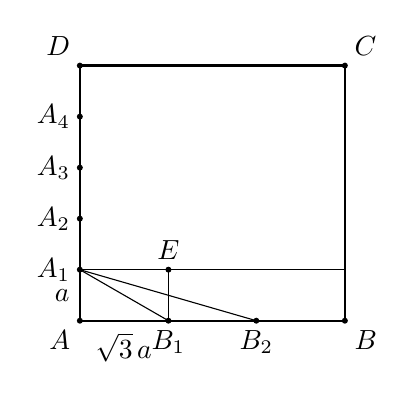
\begin{tikzpicture}[scale=0.9]
  \coordinate (A) at (0,0);
  \coordinate (B) at (3.74,0);
  \coordinate (C) at (3.74,3.6);
  \coordinate (D) at (0,3.6);
  \coordinate (A1) at (0,0.72);
  \coordinate (A2) at (0,1.44);
  \coordinate (A3) at (0,2.16);
  \coordinate (A4) at (0,2.88);
  \coordinate (B1) at (1.25,0);
  \coordinate (B2) at (2.49,0);
  \coordinate (E) at (1.25,0.72);
  \coordinate (G) at (3.74,0.72);
  \draw[thick] (A)--(B)--(C)--(D)--cycle;
  \draw[thin] (A1)--(G);
  \draw[thin] (A1)--(B1);
  \draw[thin] (A1)--(B2);
  \draw[thin] (B1)--(E);
  \fill (A) circle (1.2pt) node[below left] {$A$};
  \fill (B) circle (1.2pt) node[below right] {$B$};
  \fill (C) circle (1.2pt) node[above right] {$C$};
  \fill (D) circle (1.2pt) node[above left] {$D$};
  \fill (A1) circle (1.2pt) node[left] {$A_1$};
  \fill (A2) circle (1.2pt) node[left] {$A_2$};
  \fill (A3) circle (1.2pt) node[left] {$A_3$};
  \fill (A4) circle (1.2pt) node[left] {$A_4$};
  \fill (B1) circle (1.2pt) node[below] {$B_1$};
  \fill (B2) circle (1.2pt) node[below] {$B_2$};
  \fill (E) circle (1.2pt) node[above] {$E$};
  \node at (0.62,-0.38) {$\sqrt3\,a$};
  \node at (-0.25,0.36) {$a$};
\end{tikzpicture}
\end{center}
\nopagebreak[4]
\Needspace{4\baselineskip}
\textbf{解析}

\gksubpart{（1）}

三位数共有 $9\times10^2=900$ 个（百位不为 0）。其中：

三位数字互不相同的有 $9\times9\times8=648$ 个（百位 9 种，十位可与百位不同取 9 种，个位 8 种）；

三个数字都相同的有 $9$ 个。

\Needspace{5\baselineskip}
所以含有两个重复数字（恰有两位相同）的三位数为

\nopagebreak[4]
\[
9\times100-9\times9\times8-9=900-648-9=243\ (\text{\text{个}}).
\]

\begin{gktip}
\textbf{复核}：直接构造计数：重复数字取 $1\sim9$ 共 9 种，另一数字取其余 9 种，三个位置中选两个放重复数字共 3 种，$9\times9\times3=243$，两法一致。（重复数字为 0 的情形不能构成三位数，故重复数字只有 9 种。）
\end{gktip}

\gksubpart{（2）}

用数学归纳法证明 $x^n-y^n$ 能被 $x-y$ 整除（$n$ 为自然数）。

$1^\circ$ 当 $n=1$ 时，$x^1-y^1=x-y$ 显然能被 $x-y$ 整除，命题为真。

\Needspace{5\baselineskip}
$2^\circ$ 设当 $n=k$ 时命题为真，即 $x^k-y^k$ 能被 $x-y$ 整除。则当 $n=k+1$ 时，

\nopagebreak[4]
\[
x^{k+1}-y^{k+1}
=x^{k+1}-x^ky+x^ky-y^{k+1}
=x^k(x-y)+y(x^k-y^k).
\]

第一项含因式 $x-y$，第二项由归纳假设能被 $x-y$ 整除，所以 $x^{k+1}-y^{k+1}$ 能被 $x-y$ 整除，命题当 $n=k+1$ 时也为真。

综上，命题对一切自然数 $n$ 均为真。

\textbf{附加题 9}

\Needspace{4\baselineskip}
\textbf{解析}

\Needspace{5\baselineskip}
如图，设 $A$ 为原点，$AB$ 为 $x$ 轴正向，$AD$ 为 $y$ 轴正向，则

\nopagebreak[4]
\[
A=(0,0),\quad
B=(3\sqrt3\,a,0),\quad
C=(3\sqrt3\,a,5a),\quad
D=(0,5a),
\]

\nopagebreak[4]
\[
A_1=(0,a),\ A_2=(0,2a),\ A_3=(0,3a),\ A_4=(0,4a);
\qquad
B_1=(\sqrt3\,a,0),\ B_2=(2\sqrt3\,a,0).
\]

$E$ 为过 $B_1$ 所作 $AB$ 的垂线与过 $A_1$ 所作 $AB$ 的平行线的交点（原卷第 4 页插图所示），故 $E=(\sqrt3\,a,a)$，且 $B_1E\perp A_1E$，$A_1E=\sqrt3\,a$，$B_1E=a$。
\nopagebreak[4]
\begin{center}% 1977 年安徽卷（理科）第 9 题（附加题）：矩形 ABCD 分割示意图，
% AD 边上 A1—A4 五等分（AA1=…=A4D=a），AB 边上 B1、B2 三等分（AB1=B1B2=B2B=√3a），
% 过 A1 作 AB 的平行线交 BC 于 G，E 在该线上 B1 的正上方（B1E⊥AB），
% 连线 A1B1、A1B2（按源卷第 4 页「安，加．」手绘图布局重绘）
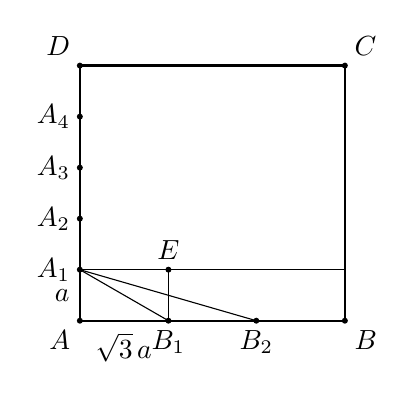
\begin{tikzpicture}[scale=0.9]
  \coordinate (A) at (0,0);
  \coordinate (B) at (3.74,0);
  \coordinate (C) at (3.74,3.6);
  \coordinate (D) at (0,3.6);
  \coordinate (A1) at (0,0.72);
  \coordinate (A2) at (0,1.44);
  \coordinate (A3) at (0,2.16);
  \coordinate (A4) at (0,2.88);
  \coordinate (B1) at (1.25,0);
  \coordinate (B2) at (2.49,0);
  \coordinate (E) at (1.25,0.72);
  \coordinate (G) at (3.74,0.72);
  \draw[thick] (A)--(B)--(C)--(D)--cycle;
  \draw[thin] (A1)--(G);
  \draw[thin] (A1)--(B1);
  \draw[thin] (A1)--(B2);
  \draw[thin] (B1)--(E);
  \fill (A) circle (1.2pt) node[below left] {$A$};
  \fill (B) circle (1.2pt) node[below right] {$B$};
  \fill (C) circle (1.2pt) node[above right] {$C$};
  \fill (D) circle (1.2pt) node[above left] {$D$};
  \fill (A1) circle (1.2pt) node[left] {$A_1$};
  \fill (A2) circle (1.2pt) node[left] {$A_2$};
  \fill (A3) circle (1.2pt) node[left] {$A_3$};
  \fill (A4) circle (1.2pt) node[left] {$A_4$};
  \fill (B1) circle (1.2pt) node[below] {$B_1$};
  \fill (B2) circle (1.2pt) node[below] {$B_2$};
  \fill (E) circle (1.2pt) node[above] {$E$};
  \node at (0.62,-0.38) {$\sqrt3\,a$};
  \node at (-0.25,0.36) {$a$};
\end{tikzpicture}
\end{center}
\nopagebreak[4]
记 $\alpha=\angle B_1A_1E$，$\beta=\angle B_2A_1E$，$\gamma=\angle BDC$。

\textbf{方法一（三角）}

在 $\mathrm{Rt}\triangle A_1EB_1$ 中，$\tan\alpha=\dfrac{B_1E}{A_1E}=\dfrac{a}{\sqrt3\,a}=\dfrac{\sqrt3}{3}$，$\alpha$ 为锐角，故 $\alpha=\dfrac{\pi}{6}$。

\Needspace{5\baselineskip}
在 $\mathrm{Rt}\triangle A_1B_2E'$ 中（$E'$ 为 $B_2$ 在直线 $A_1E$ 上的垂足，$A_1E'=2\sqrt3\,a$，$B_2E'=a$）：

\nopagebreak[4]
\[
\tan\beta=\frac{a}{2\sqrt3\,a}=\frac{\sqrt3}{6}.
\]

\Needspace{5\baselineskip}
因 $DC\parallel AB$，由内错角相等，$\gamma=\angle BDC=\angle ABD$，而在 $\mathrm{Rt}\triangle ABD$ 中

\nopagebreak[4]
\[
\tan\angle ABD=\frac{AD}{AB}=\frac{5a}{3\sqrt3\,a}=\frac{5\sqrt3}{9},
\]

\Needspace{5\baselineskip}
故

\nopagebreak[4]
\[
\tan\gamma=\frac{5\sqrt3}{9}.
\]

\Needspace{5\baselineskip}
于是由两角和的正切公式：

\nopagebreak[4]
\[
\tan(\beta+\gamma)=\frac{\tan\beta+\tan\gamma}{1-\tan\beta\tan\gamma}
=\frac{\dfrac{\sqrt3}{6}+\dfrac{5\sqrt3}{9}}{1-\dfrac{\sqrt3}{6}\cdot\dfrac{5\sqrt3}{9}}
=\frac{\dfrac{13\sqrt3}{18}}{1-\dfrac{5}{18}}
=\frac{\dfrac{13\sqrt3}{18}}{\dfrac{13}{18}}
=\sqrt3.
\]

\Needspace{5\baselineskip}
因 $0\leqslant\beta+\gamma<\pi$ 且 $\tan(\beta+\gamma)=\sqrt3>0$，故 $\beta+\gamma=\dfrac{\pi}{3}$。所以

\nopagebreak[4]
\[
\alpha+\beta+\gamma=\frac{\pi}{6}+\frac{\pi}{3}=\frac{\pi}{2},
\]

\Needspace{5\baselineskip}
即

\nopagebreak[4]
\[
\angle B_1A_1E+\angle B_2A_1E+\angle BDC=\frac{\pi}{2}.
\]

\textbf{方法二（代数）}

\Needspace{5\baselineskip}
以 $A$ 为原点、$AB$ 为 $x$ 轴正向、$AD$ 为 $y$ 轴正向建立直角坐标系，用复数表示向量。作 $B_1E\perp A_1E$、$B_2F\perp A_1F$（$E\text{、}F$ 分别为过 $B_1\text{、}B_2$ 的垂线与过 $A_1$ 而平行于 $AB$ 的直线的交点），考察向量 $\overrightarrow{AE}$、$\overrightarrow{AF}$、$\overrightarrow{AC}$ 所表示的复数：

\nopagebreak[4]
\[
z_1=\sqrt3\,a+ai,
\qquad
z_2=2\sqrt3\,a+ai,
\qquad
z_3=3\sqrt3\,a+5ai.
\]

\Needspace{5\baselineskip}
因 $A_1E\parallel AB$ 且 $B_1E\text{、}B_2F$ 均垂直于 $AB$，四边形 $AB_1EA_1$、$AB_2FA_1$ 均为矩形。$\angle B_1A_1E$ 与 $\angle EAB_1$ 是两个直角三角形（直角边同为 $a$ 与 $\sqrt3\,a$）中的锐角，故 $\alpha=\angle B_1A_1E=\angle EAB_1=\arg z_1$；同理 $\beta=\arg z_2$。又 $DC\parallel AB$，内错角相等，$\gamma=\angle BDC=\angle ABD$，而 $\tan\angle ABD=\dfrac{AD}{AB}=\dfrac{5a}{3\sqrt3\,a}$，恰为 $z_3$ 的辐角的正切，故 $\gamma=\arg z_3$。三者均为锐角，于是

\nopagebreak[4]
\[
\alpha+\beta+\gamma=\arg z_1+\arg z_2+\arg z_3=\arg(z_1z_2z_3).
\]

\Needspace{5\baselineskip}
计算乘积：

\nopagebreak[4]
\[
\begin{aligned}
z_1z_2
&=(\sqrt3\,a+ai)(2\sqrt3\,a+ai)
=a^2(\sqrt3+i)(2\sqrt3+i)
=a^2\left(5+3\sqrt3\,i\right),
\end{aligned}
\]

\nopagebreak[4]
\[
z_1z_2z_3
=a^2\left(5+3\sqrt3\,i\right)\left(3\sqrt3+5i\right)a
=a^3\left(15\sqrt3+25i+27i-15\sqrt3\right)
=52a^3i.
\]

\Needspace{5\baselineskip}
纯虚数 $52a^3i$ 的辐角为 $\dfrac{\pi}{2}$，所以

\nopagebreak[4]
\[
\angle B_1A_1E+\angle B_2A_1E+\angle BDC=\alpha+\beta+\gamma=\frac{\pi}{2}.
\]

\textbf{方法三（几何）}

作 $B_1E\perp AB$ 交直线 $A_1E$ 于 $E$，作 $B_2F\perp AB$ 交直线 $A_1E$ 于 $F$（$F$ 为 $\beta$ 之辅助点）。以 $AB$ 为对称轴作矩形 $AB_1EA_1$（连同其补矩形 $ABGA_1$，$G$ 为直线 $A_1E$ 与 $BC$ 的交点）的对称图形 $ABB_3A_5$，则 $E$ 的对称点 $E_1$ 在 $B_1$ 正下方距 $AB$ 为 $a$ 处，$E_1B_1=a$，$B_1B=2\sqrt3\,a$。

\Needspace{5\baselineskip}
第一步：在 $\mathrm{Rt}\triangle A_1EB_1$ 中，斜边 $A_1B_1=\sqrt{(\sqrt3\,a)^2+a^2}=2a$，直角边 $B_1E=\dfrac12A_1B_1$，故

\nopagebreak[4]
\[
\alpha=\angle B_1A_1E=30^\circ.
\]

\Needspace{5\baselineskip}
第二步：$\mathrm{Rt}\triangle E_1B_1B$ 与 $\mathrm{Rt}\triangle B_2FA_1$ 的两直角边对应相等（$E_1B_1=FB_2=a$，$B_1B=A_1F=2\sqrt3\,a$），故两三角形全等，从而

\nopagebreak[4]
\[
\angle E_1BB_1=\angle B_2A_1F=\beta.
\]

\Needspace{5\baselineskip}
又因 $DC\parallel AB$，内错角相等，$\gamma=\angle BDC=\angle ABD$。所以

\nopagebreak[4]
\[
\angle E_1BD=\angle E_1BA+\angle ABD=\beta+\gamma.
\]

\Needspace{5\baselineskip}
第三步：计算 $\triangle DE_1B$ 的三边（$D=(0,5a)$，$B=(3\sqrt3\,a,0)$，$E_1$ 在 $B_1$ 下方距 $AB$ 为 $a$ 处）：

\nopagebreak[4]
\[
DE_1=\sqrt{(\sqrt3\,a)^2+(6a)^2}=\sqrt{39}\,a,
\]

\nopagebreak[4]
\[
BE_1=\sqrt{(2\sqrt3\,a)^2+a^2}=\sqrt{13}\,a,
\]

\nopagebreak[4]
\[
BD=\sqrt{(3\sqrt3\,a)^2+(5a)^2}=\sqrt{52}\,a=2\sqrt{13}\,a.
\]

\Needspace{5\baselineskip}
因

\nopagebreak[4]
\[
DE_1^2+BE_1^2=39a^2+13a^2=52a^2=BD^2,
\]

\Needspace{5\baselineskip}
由勾股定理的逆定理，$\triangle DE_1B$ 是直角三角形，$\angle DE_1B=90^\circ$。又斜边 $BD=2\sqrt{13}\,a=2\,BE_1$，即直角边 $BE_1$ 为斜边之半，故其对角 $\angle BDE_1=30^\circ$，从而

\nopagebreak[4]
\[
\angle E_1BD=60^\circ,
\qquad\text{\text{即}}\qquad
\beta+\gamma=60^\circ.
\]

\Needspace{5\baselineskip}
综合两步：

\nopagebreak[4]
\[
\angle B_1A_1E+\angle B_2A_1E+\angle BDC=\alpha+\beta+\gamma=30^\circ+60^\circ=90^\circ=\frac{\pi}{2}.
\]

\gkanswer{答案（1）：$243$ 个。}

\gkanswer{答案（2）：见解析版}

\end{answer}